% !TEX root = atlas_iros_16.tex
%%%%%%%%%%%%%%%%%%%%%%%%%%%%%%%%%%%%%%%%%%%%%%%%%%%%%%%%%%%%%%%%%%%%%%%%%%%%%%%%
\section{\large Modeling and Identification}
\label{sec:advance}

In this section we shortly review the system modeling and enhanced impedance controller approach (\ref{sec:advance_controller}), modifications to the momentum-based disturbance observer to include wrist wrench measurements (\ref{sec:advance_observer}), compensation of modeling errors and collision handling (\ref{sec:friction_comp_and_collDet}), and an identification scheme that iteratively estimates friction characteristics and rigid body parameters (\ref{sec:advance_ident}).

\subsection{System Model and Joint Impedance Controller}
\label{sec:advance_controller}
This work focuses on the 7R type serial chain arms of the Boston Dynamics humanoid robot Atlas, see Fig.~\ref{fig:StickCollisionPhoto}.
The arms employ a hybrid actuation concept where the first four joints (shz, shx, ely, elx) are hydraulic, and the wrist joints (wry, wrx, wry2) are driven by electromechanical gear drives.
We assume the standard fixed-base rigid joint arm model 
\begin{equation}
\bm{M(\bm{q})}\ddot{\bm{q}}+\bm{C}(\bm{q},\dot{\bm{q}})\dot{\bm{q}}+\bm{g}(\bm{q})=\bm{\tau}_\mathrm{m}-\bm{\tau}_\mathrm{f}+\bm{\tau}_\mathrm{ext}
\label{eqn:invdyn}
\end{equation}
with generalized joint position $\bm{q} \in \mathbb{R}^{n_\mathrm{j}}$ ($n_\mathrm{j}$ being the number of joints), positive definite and symmetric inertia matrix $\bm{M}(\bm{q})$, centrifugal and Coriolis matrix $\bm{C}(\bm{q}, \dot{\bm{q}})$, gravity torque vector $\bm{g}(\bm{q})$, actuator torques $\bm{\tau}_\mathrm{m}$, friction torques $\bm{\tau}_\mathrm{f}$ and external torques $\bm{\tau}_\mathrm{ext}$. 
The friction torque $\bm{\tau}_\mathrm{f}$ is composed of the motor side friction $\bm{\tau}_{\mathrm{f},\theta}$ and the link side friction $\bm{\tau}_{\mathrm{f},q}$.
Both hydraulic and electromechanic actuators are considered as ideal torque sources, generating a motor torque $\bm{\tau}_\mathrm{m}$, allowing a separation of the actuator dynamics from the rigid body model.

For soft-robotics control of the system we chose the joint impedance control torque $\bm{\tau}_\mathrm{d}$ to be
\begin{equation}
\begin{gathered}
\bm{\tau}_\mathrm{d}=
\bm{K}(\bm{q}_\mathrm{d}-\bm{q})+\bm{D}(\dot{\bm{q}}_\mathrm{d}-\dot{\bm{q}})+\hat{\bm{g}}(\bm{q}) % tau_I 
\\
+\hat{\bm{C}}(\bm{q},\dot{\bm{q}})\dot{\bm{q}} % tau_c
+\hat{\bm{M}}(\bm{q}_\mathrm{d})\ddot{\bm{q}}_\mathrm{d} % tau_ff
+\kappa_{\mathrm{f}} \hat{\bm{\tau}}_\mathrm{f}(\dot{\bm{q}})
-\kappa_{\varepsilon} \hat{\bm{\tau}}_\mathrm{\varepsilon}(\bm{q}, \dot{\bm{q}},\bm{\tau}_\mathrm{m})\;,
\label{eqn:controller}
\end{gathered}
\end{equation}
where $\bm{q}_\mathrm{d}, \dot{\bm{q}}_\mathrm{d}, \ddot{\bm{q}}_\mathrm{d}$ are the desired position, velocity, and acceleration, respectively. The matrices $\bm{K}=\mathrm{diag}\{k_i\}$ and $\bm{D}_\xi=\mathrm{diag}\{d_{\xi,i}\}$ denote diagonal positive definite stiffness and modal damping and $\bm{D}$ the resulting positive definite damping matrix.
$\hat{\bm{g}}$ and $\hat{\bm{C}}$ are the gravity and centrifugal/Coriolis estimates.
The inertial feedforward term makes use of the estimated inertia matrix $\hat{\bm{M}}$ as a function of the desired position $\bm{q}_\mathrm{d}$.
The compensation terms $\hat{\bm{\tau}}_\mathrm{f}(\dot{\bm{q}})$ (viscous and Coulomb friction) and $\hat{\bm{\tau}}_\mathrm{\varepsilon}(\bm{q}, \dot{\bm{q}},\bm{\tau}_\mathrm{m})$ (estimated disturbance from Sec.~\ref{sec:advance_observer}) are activated via the scalars $\kappa_{\mathrm{f}}\in \{0,1\}$ and $\kappa_{\varepsilon}\in \{0,1\}$, respectively.

Combining (\ref{eqn:invdyn}) and (\ref{eqn:controller}) leads to the closed-loop dynamics
\begin{equation}
\begin{gathered}
\bm{M(\bm{q})}\ddot{\bm{q}}-\hat{\bm{M}}(\bm{q}_\mathrm{d})\ddot{\bm{q}}_\mathrm{d}
+\bm{D}(\dot{\bm{q}}-\dot{\bm{q}}_\mathrm{d})
+\bm{K}(\bm{q}-\bm{q}_\mathrm{d})
 \\
=\bm{\tau}_\mathrm{ext}
+ \bm{\delta}
-\kappa_{\varepsilon} \hat{\bm{\tau}}_\mathrm{\varepsilon},
\label{eqn:closedloop_general}
\end{gathered}
\end{equation}
where $\bm{\delta}$ denotes lumped dynamics and friction modeling errors and errors caused by sensor drift, offsets and time delays. 
We assume these effects to be additive. 

\subsection{Disturbance Observer}
\label{sec:advance_observer}
%
\begin{figure}
\centering
\input{./figures/MechErsatzBSB/rigid_flexible_joint_struktur.pdf_tex}
\caption{Relevant torques acting along the mechanical structure for the rigid joint model (a) with link inertia $\bm{M}$ and the flexible joint model (b) with motor inertia $\bm{B}$ and motor position $\bm{\theta}$.}
\label{fig:rigid_flexible_joint_structure}
\SkipBeforeText
\end{figure}
%
Before introducing our observer design, let us shortly summarize the underlying problem of collision detection with typical hydraulic robots.
Figure~\ref{fig:rigid_flexible_joint_structure} emphasizes the friction torques that are relevant for rigid joint models in comparison to the flexible joint case.
The latter represents e.g. electromechanically actuated robots with elastic joints and torque sensing \cite{Ott2008}. 
In the former case, the total friction $\bm{\tau}_\mathrm{f}$ and external torques $\bm{\tau}_\mathrm{ext}$ act on a single body that represents both motor and link inertia and sum up to a total disturbance torque.
Thus, except under certain modeling assumptions they cannot be separated with standard proprioceptive sensing and according observer techniques. 
In the latter case, motor and link-side dynamics are coupled via the joint stiffness $\bm{K}_{\mathrm{J}}$.
Typically, this originates either from rather elastic gears such as Harmonic Drives in combination with joint torque sensors (rather high inherent stiffness $\bm{K}_{\mathrm{J}}$), or from deliberately placed spring elements as e.g. in the Series Elastic Actuation (SEA \cite{PrattWil1995}) case (rather low inherent stiffness $\bm{K}_{\mathrm{J}}$).
Since the link side friction $\bm{\tau}_{\mathrm{f},q}$ is usually low (it is mainly caused by low friction link-side bearings), it may be neglected and the link-side observer essentially estimates the true external joint torques \cite{Haddadin2014}.
Therefore, it is possible to set up two observer schemes, one for the actuator side estimating $\bm{\tau}_{\mathrm{f},\theta}$ \cite{LeTienAlbDeHir2008}, and one for the link side estimating $\bm{\tau}_\mathrm{ext}$.
Note that one can obviously set up an elastic joint model for the hydraulic case as well.
However, this would only have a similar implication if an additional joint torque sensor for decoupling would be inserted after link friction.

To be able to distinguish between internal and external effects, we extend the momentum-based disturbance observer from \cite{DeLucaMat2003,DeLucaMat2004,Haddadin2014} to include measurements of external wrenches $\medmuskip=1.3mu
\thinmuskip=1.3mu
\thickmuskip=1.3mu
\bm{\mathcal{F}}_\mathrm{ext,EE}=\begin{pmatrix}\bm{f}_{\mathrm{ext,EE}} & \bm{m}_{\mathrm{ext,EE}}\end{pmatrix}^\mathrm{T}$ that act on the end-effector, i.e. ``after'' the sensor \cite{OttHenLee2013}.
The extended residual for end-effector contacts is then defined as
%
\begin{equation}
\medmuskip=0.5mu
\thinmuskip=0.5mu
\thickmuskip=0.5mu
\hat{\bm{\tau}}_\mathrm{\varepsilon}=\bm{K}_\mathrm{o}
\left(
\hat{\bm{M}}(\bm{q})\dot{\bm{q}}
-\int\limits_0^t
 [\bm{\tau}_\mathrm{m}
 -\bm{\gamma}(\bm{q},\dot{\bm{q}})
 +\hat{\bm{\tau}}_\mathrm{\varepsilon}
 -\bm{\alpha}(\bm{q},\dot{\bm{q}})
 ]\mathrm{d}\tilde{t} 
 \right),
\label{eqn:observer}
\end{equation}
%
where $\bm{K}_\mathrm{o}=\mathrm{diag}\{k_{\mathrm{o},i}\}>\bm{0}$ is the observer gain matrix and
\begin{equation}
\medmuskip=0.05mu
\thinmuskip=0.05mu
\thickmuskip=0.05mu
\bm{\gamma}(\bm{q},\dot{\bm{q}}):=
\hat{\bm{g}}(\bm{q})
+\hat{\bm{C}}(\bm{q},\dot{\bm{q}})\dot{\bm{q}}
-\dot{\hat{\bm{M}}}(\bm{q})\dot{\bm{q}}
=
\hat{\bm{g}}(\bm{q})-\hat{\bm{C}}^\mathrm{T}(\bm{q},\dot{\bm{q}})\dot{\bm{q}}\;.
\label{eqn:gamma}
\end{equation}
Equality (\ref{eqn:gamma}) follows directly from the skew-symmetry of $\dot{\hat{\bm{M}}}(\bm{q})-2\hat{\bm{C}}(\bm{q},\dot{\bm{q}})$ \cite{DeLucaAlbHadHir2006}. 
The vector $\bm{\alpha}(\bm{q},\dot{\bm{q}})$ is defined as 
\begin{equation}
\begin{split}
\bm{\alpha}(\bm{q},\dot{\bm{q}}) :=& 
\kappa_{\mathrm{f}}\hat{\bm{\tau}}_\mathrm{f}(\dot{\bm{q}}) -\kappa_{\mathrm{ext}}\bm{\tau}_{\mathrm{ext,EE}} \\
=&
\kappa_{\mathrm{f}}\hat{\bm{\tau}}_\mathrm{f}(\dot{\bm{q}})
-\kappa_{\mathrm{ext}}\bm{J}^{\mathrm{T}}(\bm{q}) \bm{\mathcal{F}}_\mathrm{ext,EE} \; .
\end{split}
\label{eqn:observer_settings}
\end{equation}
The contact wrench $\bm{\mathcal{F}}_\mathrm{ext,EE}$ is typically measured with a load-compensated force/torque sensor in the robot wrist.
The resulting external joint torques $\bm{\tau}_{\mathrm{ext,EE}}$ are obtained by the well known mapping via the end-effector Jacobian $\bm{J}(\bm{q})$. 
Its feedback is activated via $\kappa_{\mathrm{ext}} \in \{0,1\}$. 
Note that the components of $\bm{\mathcal{F}}_\mathrm{ext,EE}$ that are in the kernel of $\bm{J}^{\mathrm{T}}(\bm{q})$ are absorbed by the structure of the robot and are not reflected in $\bm{\tau}_{\mathrm{ext,EE}}$. 

To distinguish directly measurable joint torques originating from external wrenches at the end-effector $\bm{\tau}_{\mathrm{ext,EE}}$ from joint torques caused by external wrenches at the structure $\bm{\tau}_{\mathrm{ext,links}}$ that cannot be measured by the wrist sensor, we define the total external torque vector $\bm{\tau}_{\mathrm{ext}}$ to be
\begin{equation}
\bm{\tau}_{\mathrm{ext}} := \bm{\tau}_{\mathrm{ext,EE}} + \bm{\tau}_{\mathrm{ext,links}}.
\label{eqn:extjointtorqueseparata}
\end{equation}
The true disturbance joint torque ${\bm{\tau}}_\mathrm{\varepsilon}$ for rigid joint models consists of the joint torques from (\ref{eqn:extjointtorqueseparata}) plus the error term $\bm{\delta}$ in (\ref{eqn:closedloop_general}).
%
As derived in \cite{Haddadin2014} the observed disturbance torque, also for this extended form, converges element-wise with first order dynamics (presented in frequency domain)
\begin{equation}
\hat{\tau}_{\mathrm{\varepsilon},i}=
\frac{k_{\mathrm{o},i}}{s+k_{\mathrm{o},i}}
\left(\tau_{\mathrm{ext,EE},i}(1-\kappa_{\mathrm{ext}})
+ \tau_{\mathrm{ext,link},i}
+ \delta_{i}
\right)
\label{eqn:disttorqueconvergence}
\end{equation}
where $1/k_{\mathrm{o},i}$ is the time constant.
%
\begin{figure}
\centering
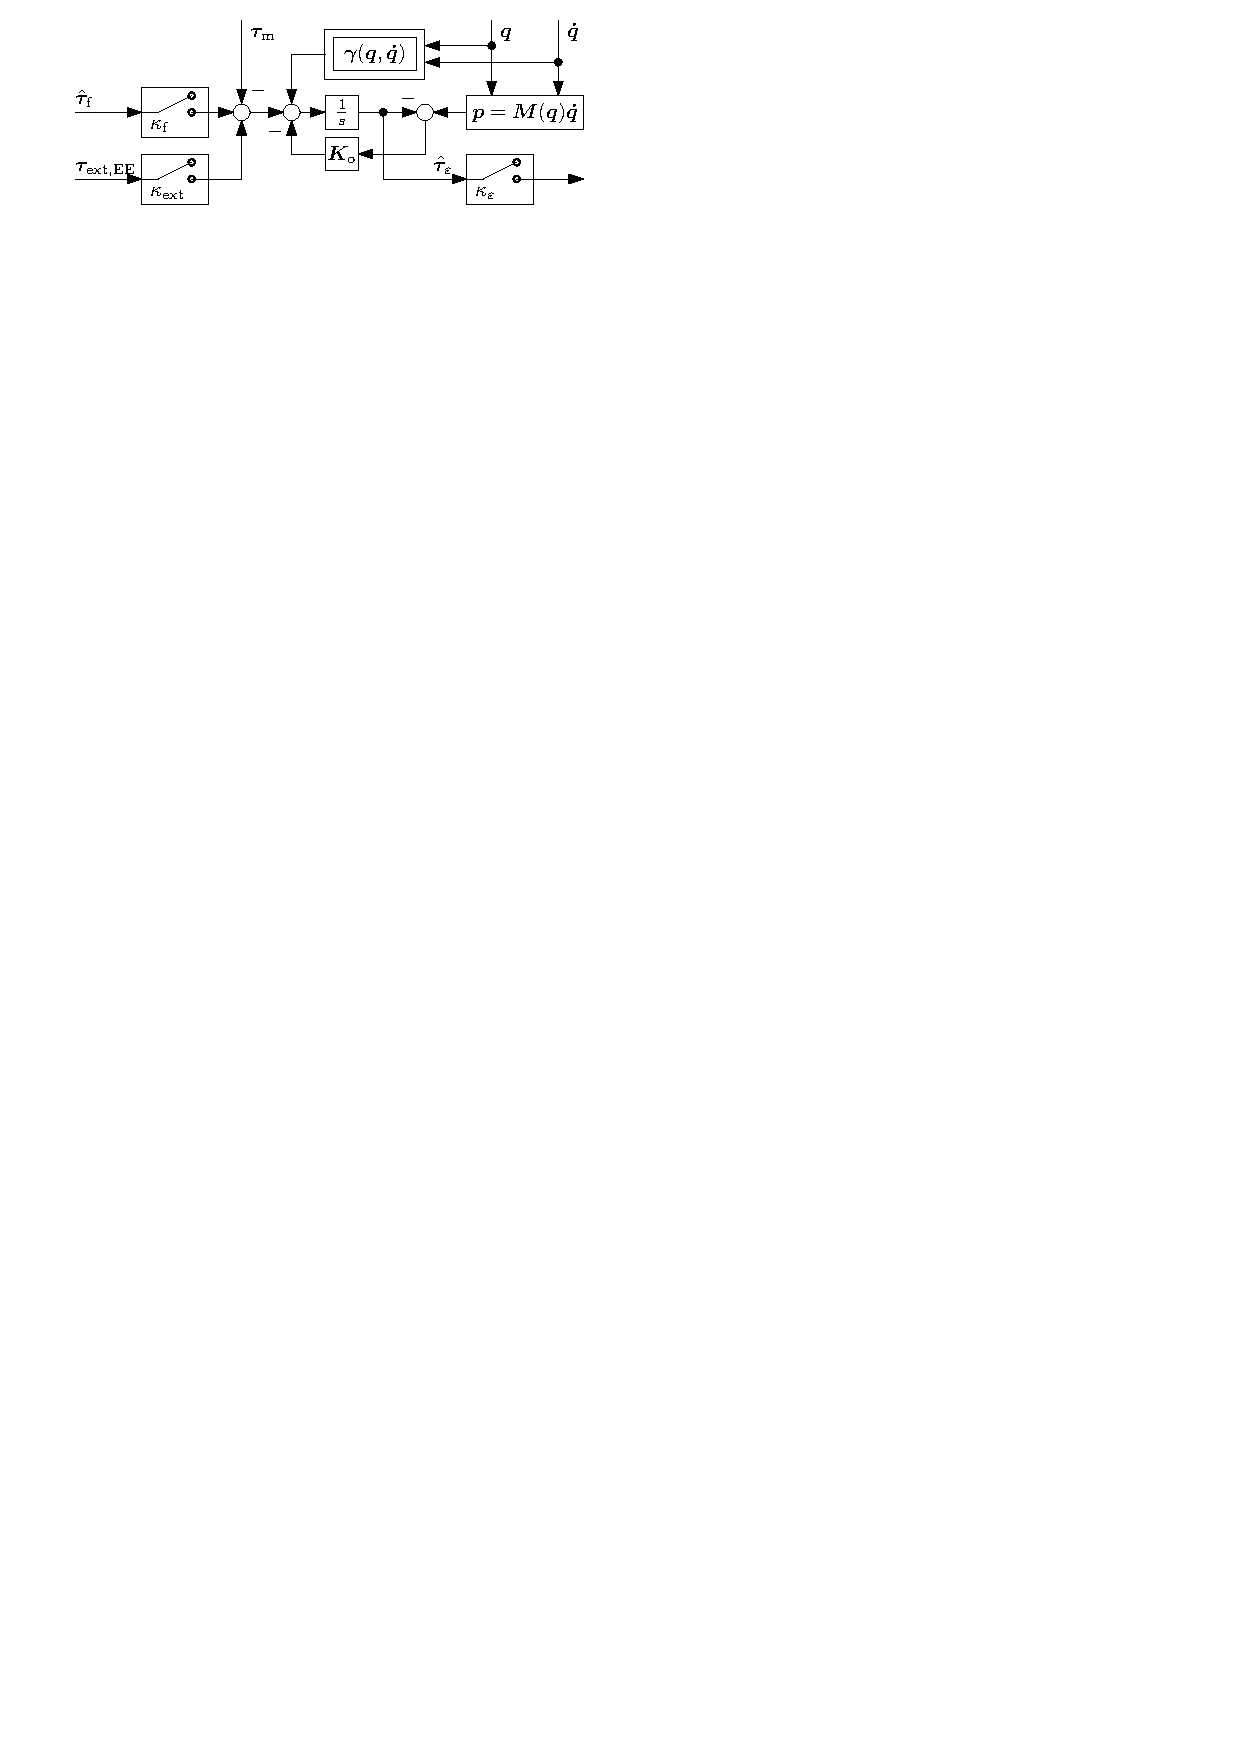
\includegraphics{./figures/ObserverFlowChart/observer_scheme}
\caption{Flowchart of the proposed observer structure.}
\label{fig:observer_flowchart}
\SkipBeforeText
\end{figure}
%
Figure~\ref{fig:observer_flowchart} depicts an overview of the overall observer structure.

In the next section, we outline how this extended disturbance observer is used to compensate for model errors and detect collisions simultaneously. 

\subsection{Compensation of Model Errors and Collision Detection}
\label{sec:friction_comp_and_collDet}

Assuming $\bm{\tau}_\mathrm{ext}$ to have slower dynamics than the observer (sufficiently large observer gain $\bm{K}_{\mathrm{o}}$).
One can approximate the disturbance torque as
\mbox{$\hat{\bm{\tau}}_\mathrm{\varepsilon}\approx
\left(\bm{\tau}_\mathrm{ext,EE}(1-\kappa_{\mathrm{ext}})
+ \bm{\tau}_\mathrm{ext,link}
+ \bm{\delta}
\right)$}.
Therefore, one obtains from equation (\ref{eqn:closedloop_general})
\begin{equation}
\begin{split}
\bm{M(\bm{q})}\ddot{\bm{q}}-\hat{\bm{M}}(\bm{q}_\mathrm{d})\ddot{\bm{q}}_\mathrm{d}
+\bm{D}(\dot{\bm{q}}-\dot{\bm{q}}_\mathrm{d})
+\bm{K}(\bm{q}-\bm{q}_\mathrm{d})\\
= \bm{\tau}_\mathrm{ext}+\bm{\delta}
-\kappa_{\varepsilon}\left(
  \bm{\tau}_\mathrm{ext,EE}(1-\kappa_{\mathrm{ext}})
+ \bm{\tau}_\mathrm{ext,link}
+ \bm{\delta}
\right)\;.
\end{split}
\label{eqn:closed_loop_converged}
\end{equation}
The trajectory tracking performance can thus be improved significantly by using the disturbance compensation with $\kappa_{\varepsilon}=1$ in (\ref{eqn:controller}) and $\kappa_\mathrm{ext}=0$ in (\ref{eqn:observer_settings}), as this would eliminate model inaccuracies $\bm{\delta}$. 
The obvious drawback would be the loss of compliance w.r.t. external torques, since equation (\ref{eqn:closed_loop_converged}) becomes
\begin{equation}
\bm{M(\bm{q})}\ddot{\bm{q}}-\hat{\bm{M}}(\bm{q}_\mathrm{d})\ddot{\bm{q}}_\mathrm{d}
+\bm{D}(\dot{\bm{q}}-\dot{\bm{q}}_\mathrm{d})
+\bm{K}(\bm{q}-\bm{q}_\mathrm{d})
= \bm{0}.
\label{eqn:compLoss}
\end{equation}
Thus, the system no longer reacts to external forces in case of precise disturbance estimates. 
This unwanted increase in stiffness could be avoided for interaction with the end-effector by exploiting wrist wrench sensing.
Setting $\kappa_{\varepsilon}=1$ in (\ref{eqn:controller}) and $\kappa_{\mathrm{ext}}=1$ in (\ref{eqn:observer_settings}), the closed loop behavior (\ref{eqn:closedloop_general}) becomes
%
\begin{equation}
\medmuskip=3mu
\thinmuskip=3mu
\thickmuskip=3mu
\bm{M(\bm{q})}\ddot{\bm{q}}-\hat{\bm{M}}(\bm{q}_\mathrm{d})\ddot{\bm{q}}_\mathrm{d}
+\bm{D}(\dot{\bm{q}}-\dot{\bm{q}}_\mathrm{d})
+\bm{K}(\bm{q}-\bm{q}_\mathrm{d})=
\bm{\tau}_\mathrm{ext,EE}\;.
\label{eqn:regainComp}
\end{equation}
This scheme has similarities to the one proposed in \cite{Oh1999} and will be termed disturbance compensation (DC) with external forces compliance (EFC) from now on. A qualitative comparison for the different settings of $\kappa_{\varepsilon}$ and $\kappa_\mathrm{ext}$ is shown in the Table of Fig.~\ref{fig:ReactionScheme}.
%

In summary, it is possible to 
%
\begin{enumerate}
\item detect end-effector contacts with the inertia compensated wrench sensor,
\item detect contacts along the entire robot structure beyond a tolerance band with the extended observer,
\item render end-effector compliance while having stiff behavior for contacts along the robot structure.
\end{enumerate}

The missing compliance for link collisions can still be encountered by switching to compliance control as soon as a link collision is detected. 

Using the above observer, we implemented a simple collision detection scheme that is based on a constant disturbance joint torque threshold ${\bm{\zeta}}$.
%
\begin{equation}
\text{CollDet}=
\begin{cases}
    1,& \text{if } \hat{\bm{\tau}}_{\varepsilon} > {\bm{\zeta}} \text{ (component wise)}\\
    0,& \text{otherwise}
\end{cases}
\label{eqn:CollDet}
\end{equation}
For (\ref{eqn:CollDet}) to work properly, one has to solve the trade-off between robustness and convergence speed of the observer.
The first order observer dynamics in (\ref{eqn:disttorqueconvergence}) with time constant $1/k_{\mathrm{o},i}$ makes the collision detection robust against sensor noise and peaks, as long as $\bm{K}_{\mathrm{o}}$ is not chosen too large.
However, large $\bm{K}_{\mathrm{o}}$ leads to faster convergence of $\hat{\bm{\tau}}_\mathrm{\varepsilon}$ to $\bm{\tau}_\mathrm{ext}$.

\begin{figure}
\centering
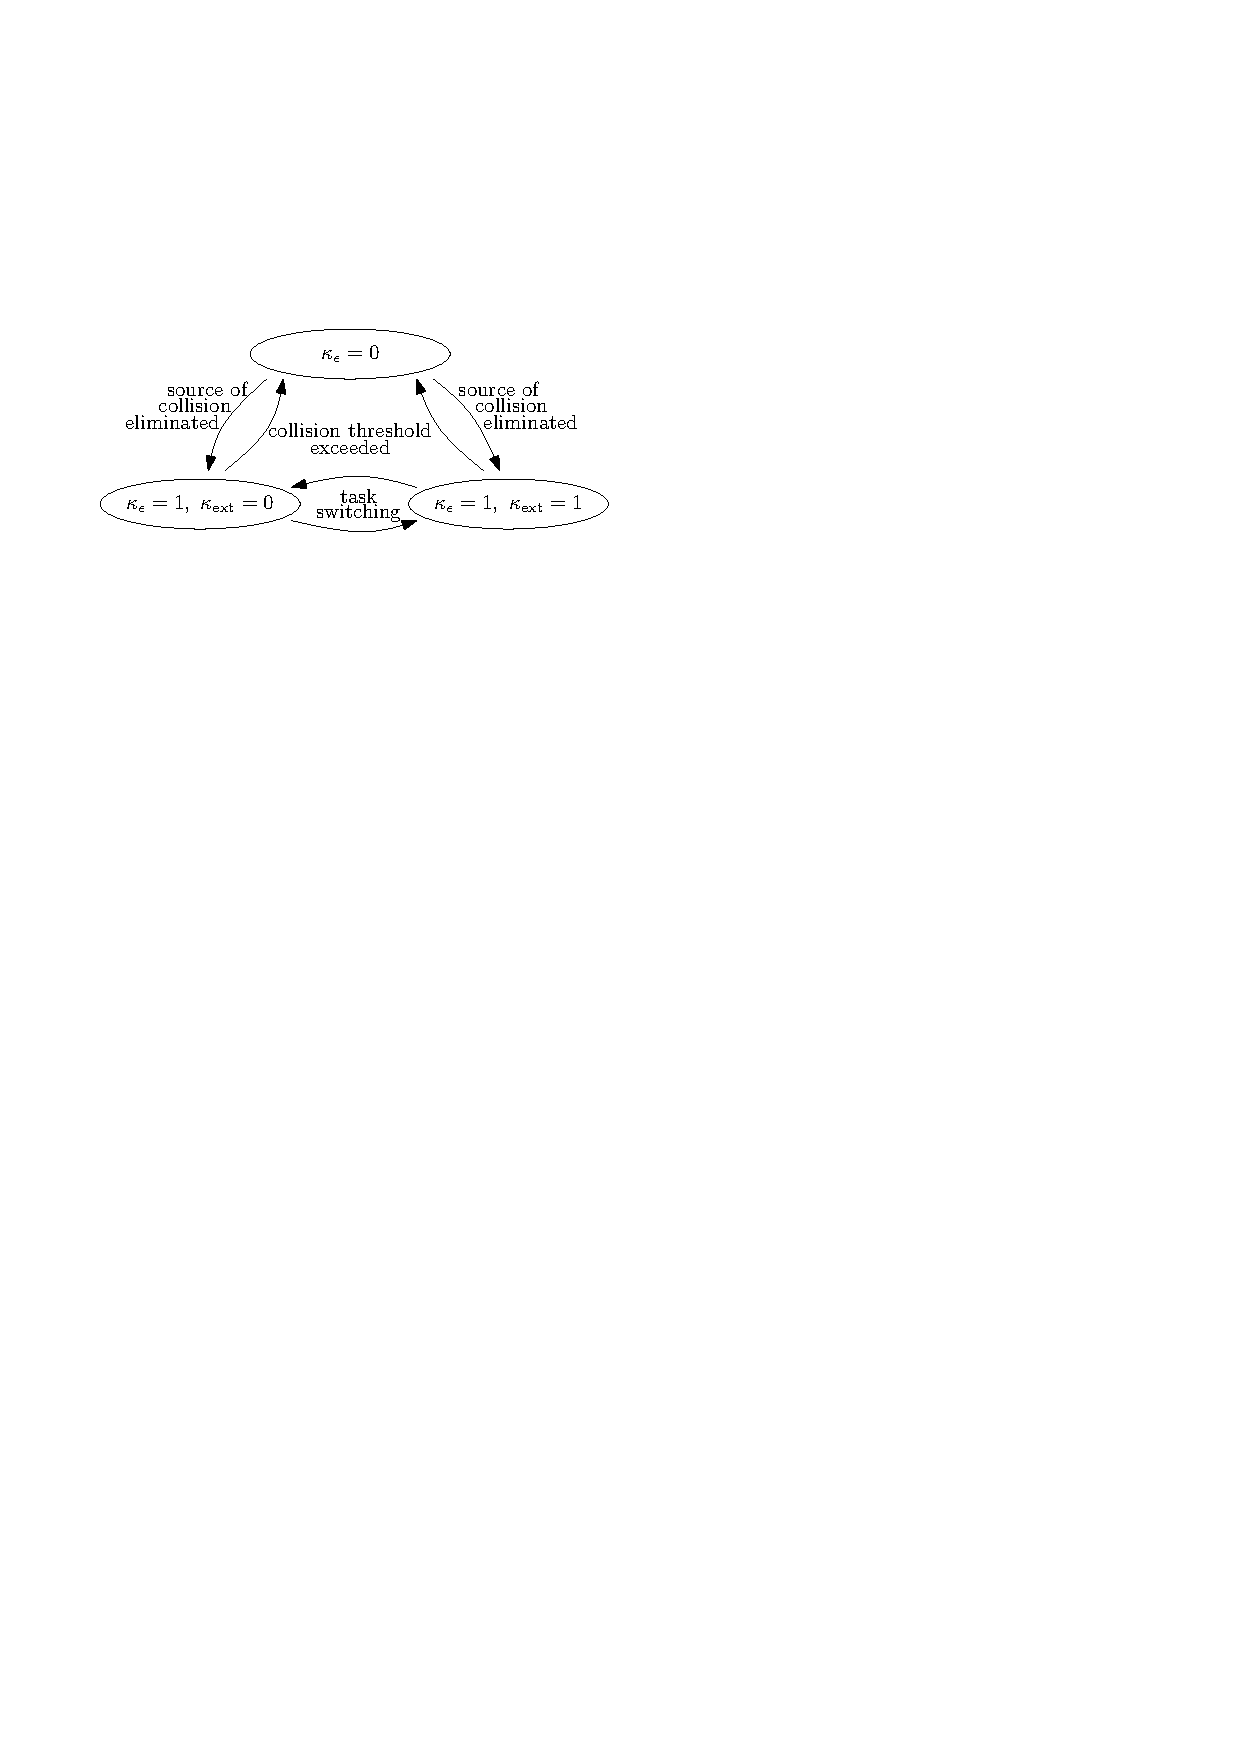
\includegraphics[scale=0.999]{./figures/ReactionScheme/reaction_scheme}
\SkipBeforePicture
\begin{center}\footnotesize
\begin{tabular}{|l|c|c|c|}
\hline
Property & $\kappa_{\varepsilon}=0$ & $\medmuskip=0mu
\thinmuskip=0mu \thickmuskip=0mu \kappa_{\varepsilon}=1, \kappa_{\mathrm{ext}}=0$ & $\medmuskip=0mu \thinmuskip=0mu \thickmuskip=0mu \kappa_{\varepsilon}=\kappa_{\mathrm{ext}}=1$ \\
\hline
Increased accuracy      & \no & \ok & \ok \\
\hline
End-effector compliance  & \ok & \no & \ok \\
\hline
Link compliance          & \ok & \no & \no \\
\hline
Closed-loop behavior & (\ref{eqn:closedloop_general}) & (\ref{eqn:compLoss}) & (\ref{eqn:regainComp}) \\
\hline
\end{tabular}
\end{center}
\SkipBeforePicture
\caption{Context sensitive control and reaction scheme and comparison between different setups of controller (\ref{eqn:controller}).
Control mode \mbox{$\kappa_\mathrm{ext}=1$} is used for tasks which need end-effector compliance, \mbox{$\kappa_\mathrm{ext}=0$} for tasks which do not. When a collision is detected, the controller switches into compliant mode ($\kappa_\varepsilon=0$).}
\label{fig:ReactionScheme}
\SkipBeforeText
\end{figure}

For collision reaction, in this work, we switch to gravity compensation mode \cite{Haddadin2014}:
\begin{equation}
\bm{\tau}_\mathrm{d}=
\begin{cases}
    \hat{\bm{g}}(\bm{q}),& \text{if CollDet}=1 \\
    \bm{\tau}_\mathrm{d} \text{ from (\ref{eqn:controller})},& \text{otherwise}\;.
\end{cases}
\label{eqn:CollReact}
\end{equation}
%
Another possibility would be to implement the scheme depicted in Fig.~\ref{fig:ReactionScheme}.
It uses the three control modes in the table in a context sensitive manner.
For example, for grasping objects end-effector compliance and high position accuracy is needed, therefore \mbox{$\kappa_\varepsilon=1$} and \mbox{$\kappa_\mathrm{ext}=1$} is used. For moving objects of unknown weight, end-effector compliance is not wanted and therefore \mbox{$\kappa_\mathrm{ext}=1$} is used.
Finally, if the collision threshold is exceeded, the robot switches into full compliant mode (\mbox{$\kappa_\varepsilon=0$}) to avoid damage.

Next, we outline our system identification and friction modeling approach.


